\chapter{Постановка задачи}
\label{cha:ch_1}

Целью работы является реализация нового Бендера, включая его схлопывание
(см. рис.~\ref{fig:3-1-shrink}). Требуется:

\begin{enumerate}
    \item Разработать архитектуру для нового Бендера:
    \begin{enumerate}
        \item Декомпозировать задачу,
        \item Описать базовый макет,
        \item Описать архитектуру компонента;
    \end{enumerate}
    \item Реализовать новый Бендер, решив каждую подзадачу,
    появившуюся в результате декомпозиции.
\end{enumerate}

\begin{figure}[h]
    \center{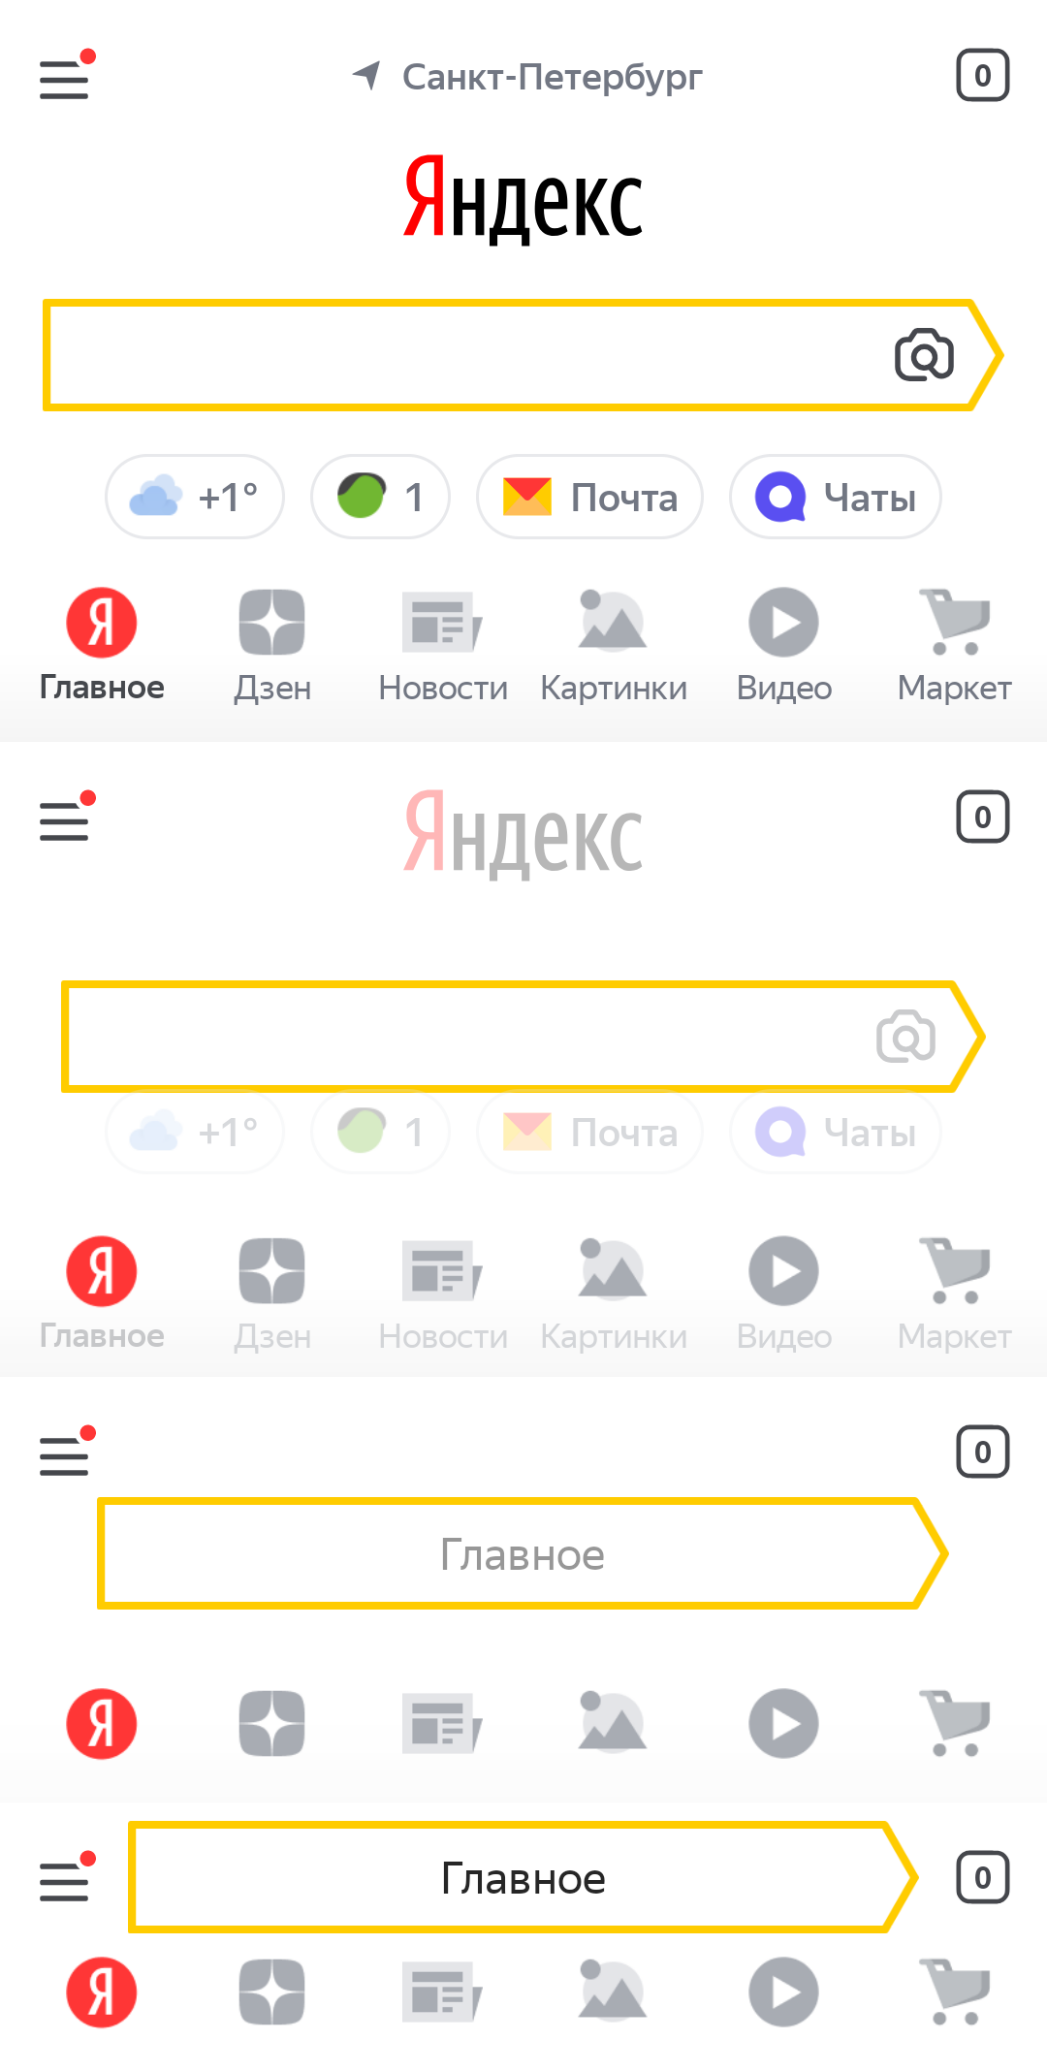
\includegraphics[scale=0.3]{3-1-shrink}}
    \caption{Процесс схлопывания Бендера}
    \label{fig:3-1-shrink}
\end{figure}
